\chapter{Navigations-Problem}\label{sec:NavigationProblem}
Wir betrachten zunächst ein Landschaftsnavigationsproblem. Der Agent soll in einer zufällig generierten Landschaft unterschiedliche Aufgaben lösen.

%% Das Environment
\section{Das Environment}

Das Environment für diese Experimentreihe bildet eine Gebirgslandschaft, über der ein Raster liegt, worauf sich der Agent bewegen soll. Hierbei soll jeder Punkt auf dem Raster eine Höhe besitzen. Außerdem soll die Landschaft zufällig generiert werden können.

Die simpelste Lösung hierfür wäre wohl, ein zweidimensionales Array mit zufälligen Zahlen zu füllen. Auf diese Weise erhält man ein für jede Koordinate eine zufällige Höhe. Wir wollen allerdings eine Landschaft erstellen, die organisch und natürlich aussieht.

% \subsection{Perlin Noise}
\paragraph{Perlin Noise}
Um dieses Ziel zu erreichen verwenden wir \textit{Perlin Noise}. Hierbei handelt es sich um eine Rauschfunktion, mit der sich sehr natürlich wirkende Texturen zufällig generieren lassen. Abbildung \ref{img:perlinNoise} zeigt eine simple Darstellung von zweidimensionaler Perlin Noise, bei der die generierten Werte über Farbwerten von Schwarz bis Weiß abgebildet werden.

\begin{figure}[h]
    \centering
    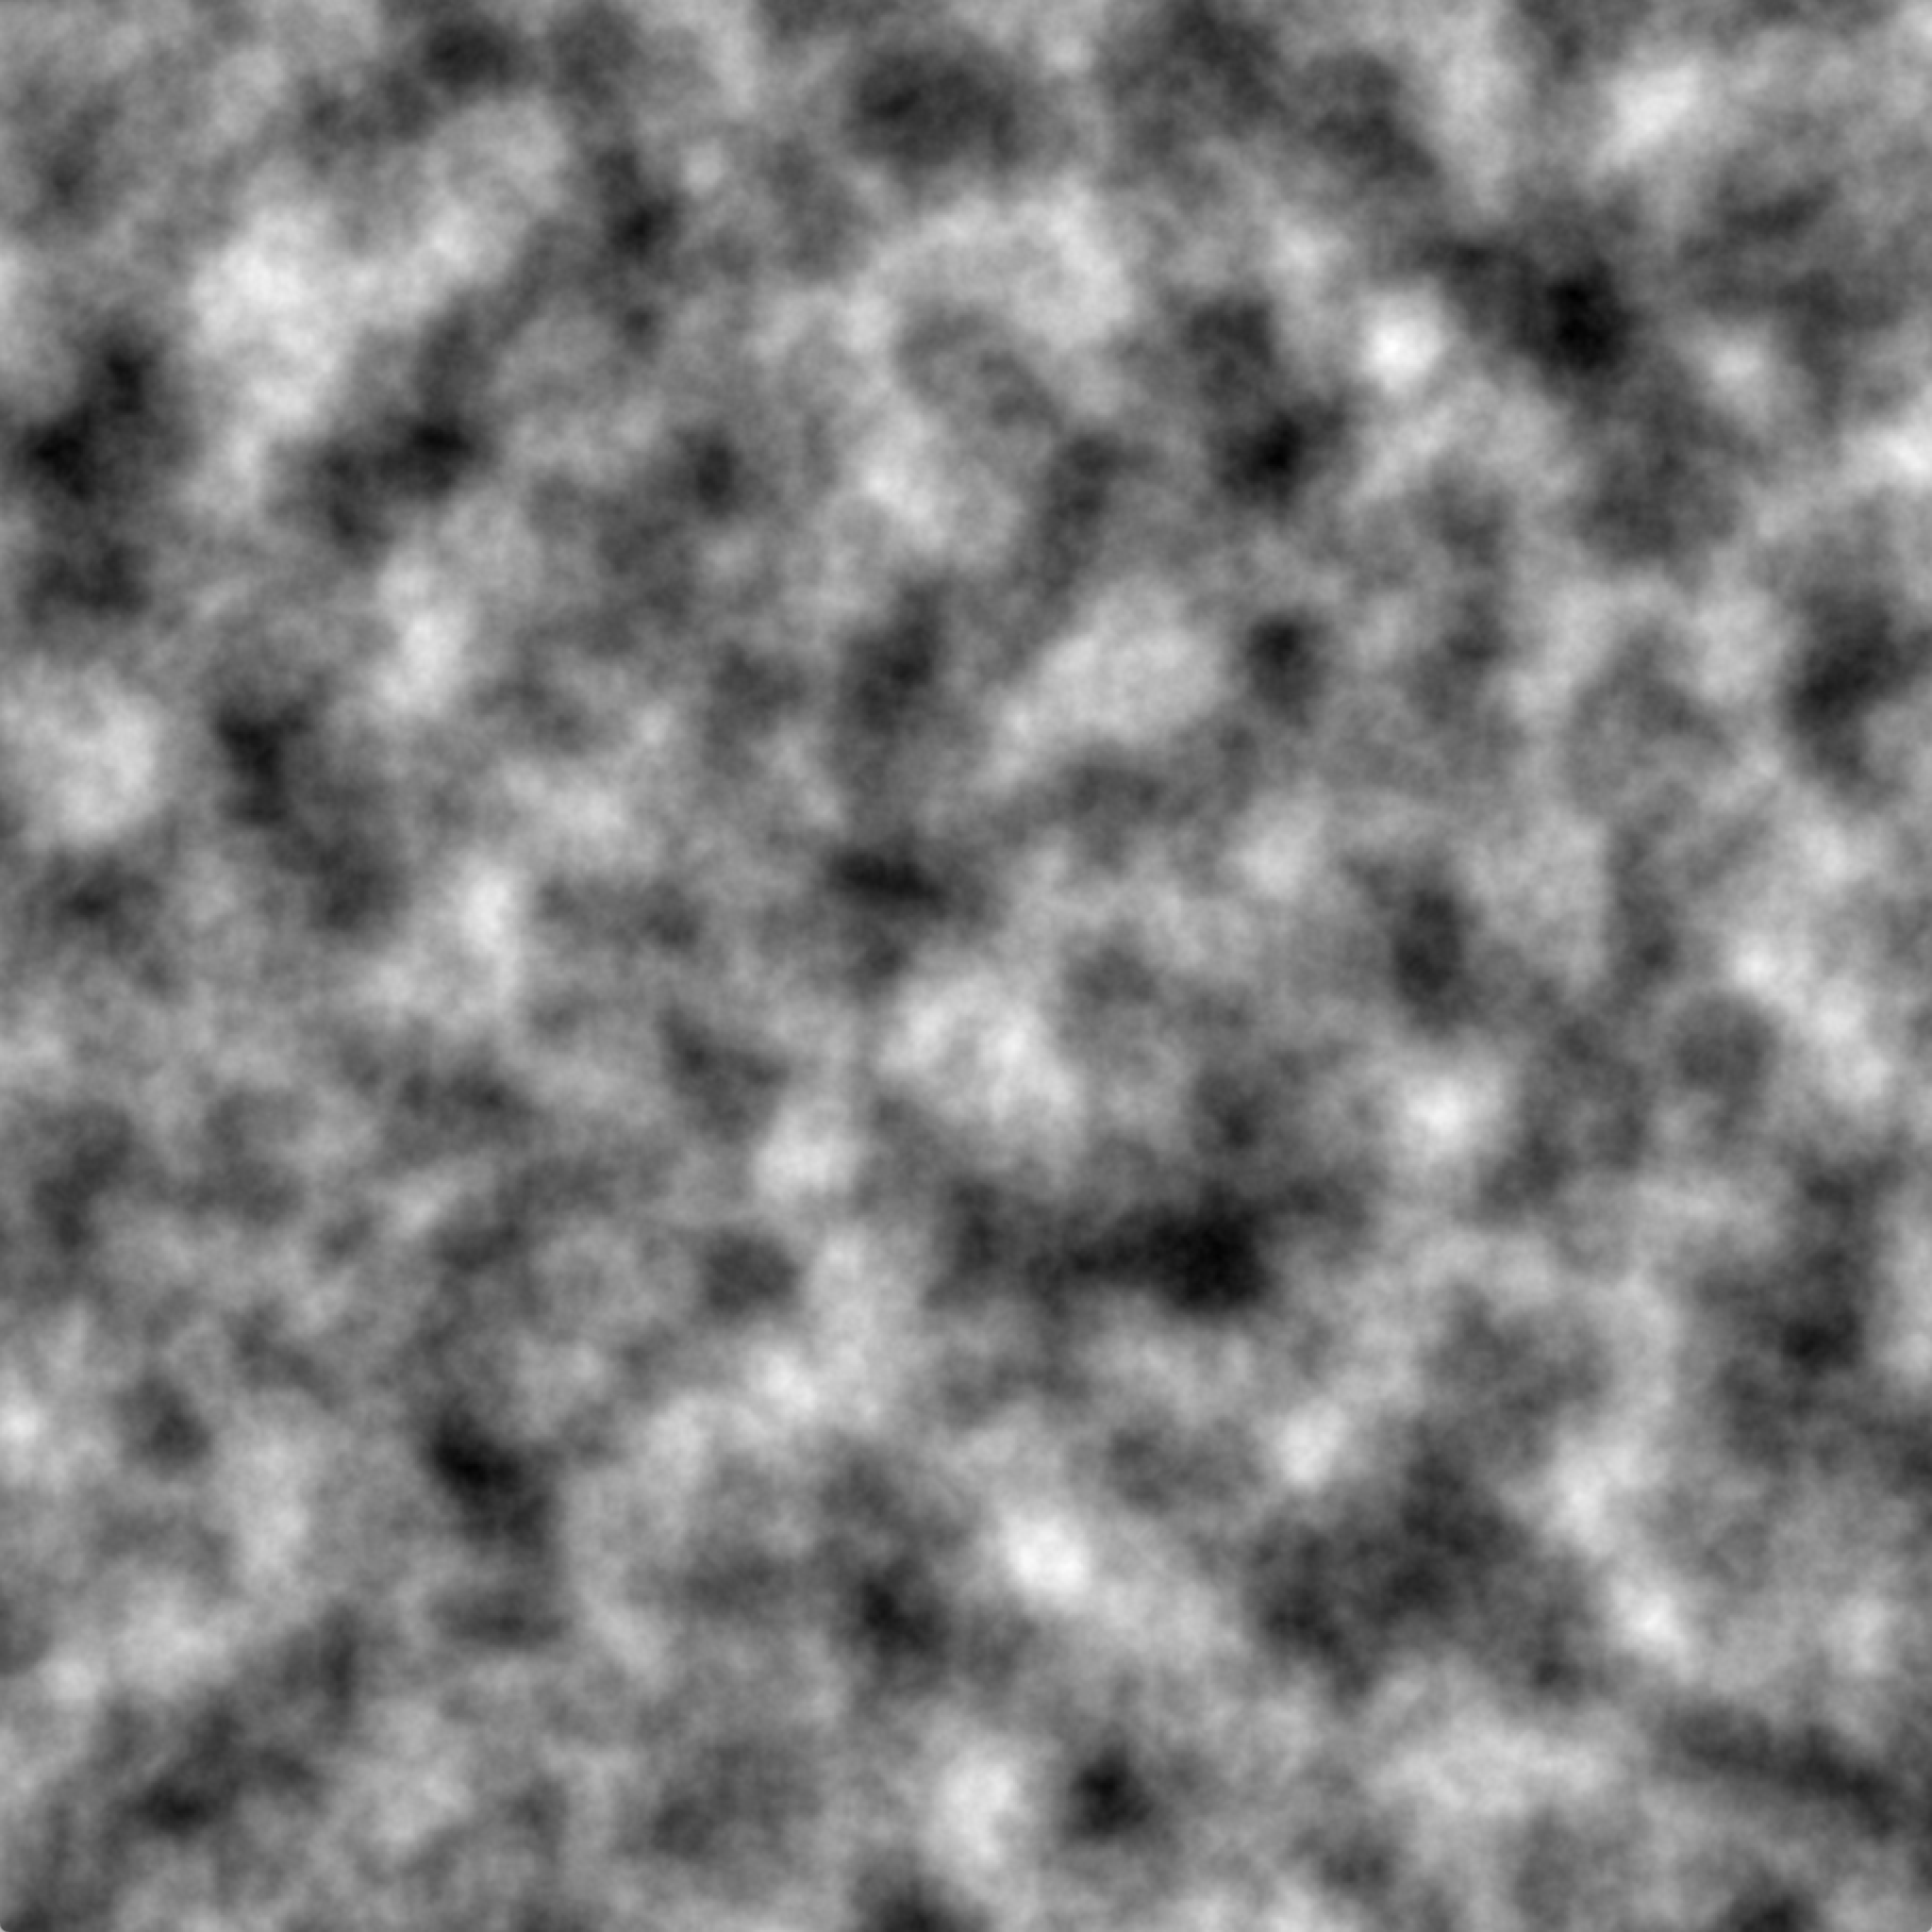
\includegraphics[width=0.5\textwidth, keepaspectratio=true]{perlin_noise.png}
    \caption{Visualisierung von zweidimensionaler Perlin Noise} \label{img:perlinNoise}
    \source{\url{https://miro.medium.com/max/2400/1*vs239SecVBaB4HvLsZ8O5Q.png}}
\end{figure}

% TODO evtl weiter ausführen
% Bei Initialisierung der Klasse werden zunächst $ x \cdot y $ Gradienten erstellt, wobei $ x $ und $ y $ entweder der Länge und der Breite des Rasters entsprechen, oder einem Bruchteil dessen, um gewissermaßen in das Rauschen \glqq hereinzuzoomen \grqq{}.

% \begin{minted}{python}
% class PerlinNoise:

%     def __init__(self, x, y):
%         x, y = math.ceil(x) + 1, math.ceil(y) + 1
%         self.gradients = []
%         for j in range(y):
%             self.gradients.append([])
%             for i in range(x):
%                 a = random.uniform(0, 1)
%                 b = math.sqrt(1 - a ** 2)
%                 c = [-1, 1][random.randint(0, 1)]
%                 d = [-1, 1][random.randint(0, 1)]
%                 self.gradients[j].append([a * c, b * d])
% \end{minted}

Perlin Noise ist nach \cite{parberry2015modeling} ein fundamentaler Algorithmus in der prozeduralen Generierung von von Terrain und somit optimal geeignet, um unsere Umgebung zu erstellen. Wir verwenden eine modifizierte Implementierung von TODO, um ein zweidimensionales Array mit zufälligen Werten zwischen -1 und 1 zu erhalten, welche wir mit einer beliebigen Höhe multiplizieren können. Je nachdem, wie stark man in die Rauschfunktion \glqq hereinzoomt \grqq{} erhält man unterschiedliche Verteilungen der Landschaft, wie man in Abbildung \ref{img:randomTerrain} erkennen kann.

\begin{figure}[h]
    \centering
    \begin{subfigure}[b]{0.49\textwidth}
        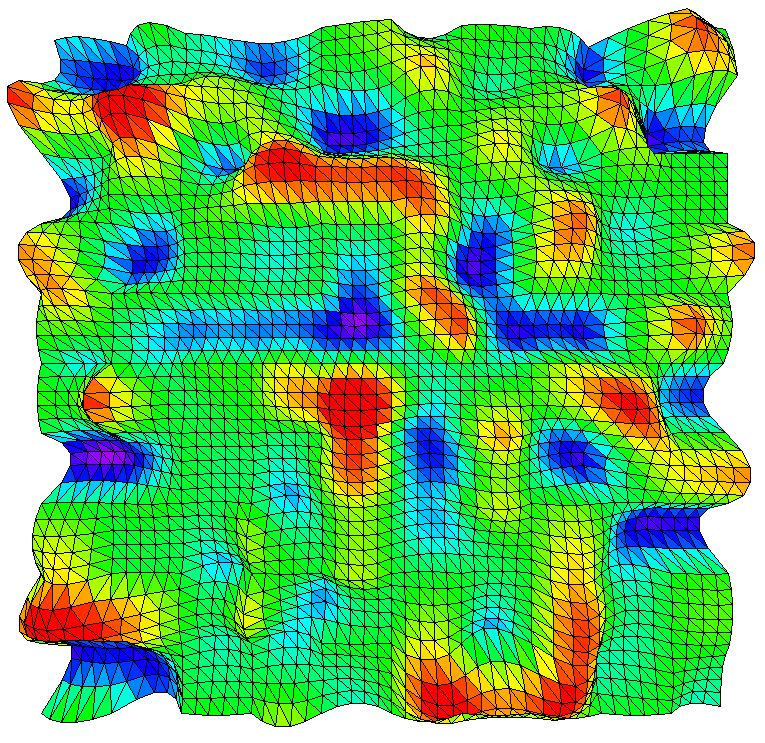
\includegraphics[width=\textwidth]{terrain_01.JPG}
        \caption{Landschaft mit niedriger Verteilung}
        \label{img:randomTerrainA}
    \end{subfigure}
    \begin{subfigure}[b]{0.49\textwidth}
        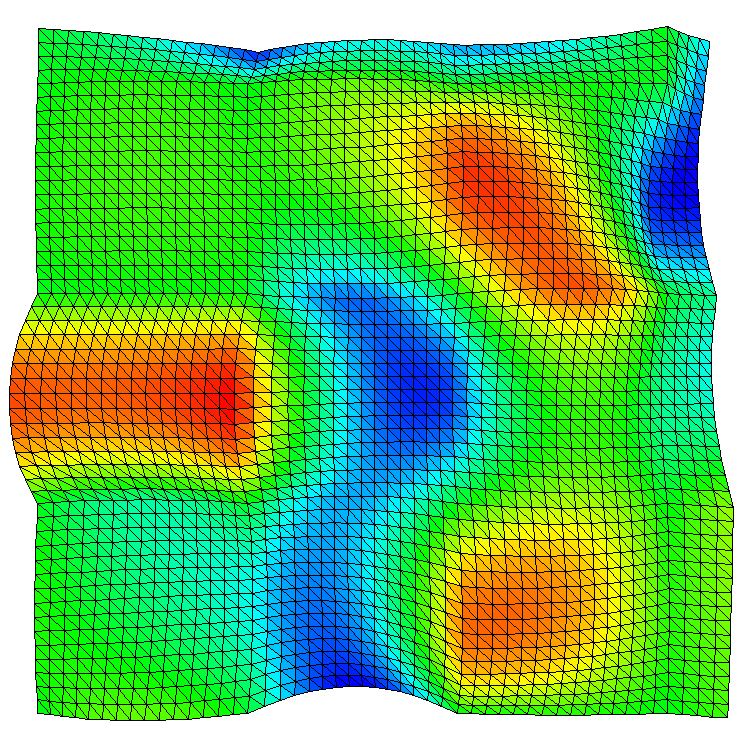
\includegraphics[width=\textwidth]{terrain_02.JPG}
        \caption{Landschaft mit hoher Verteilung}
        \label{img:randomTerrainB}
    \end{subfigure}
    \caption{Mittels Perlin Noise zufällig generierte Landschaften}
    \label{img:randomTerrain}
    % \subfigure[Figur A]{terrain_01.JPG}
    % \subfig[Figur A]{ \label{img:randomTerrainA}
    %     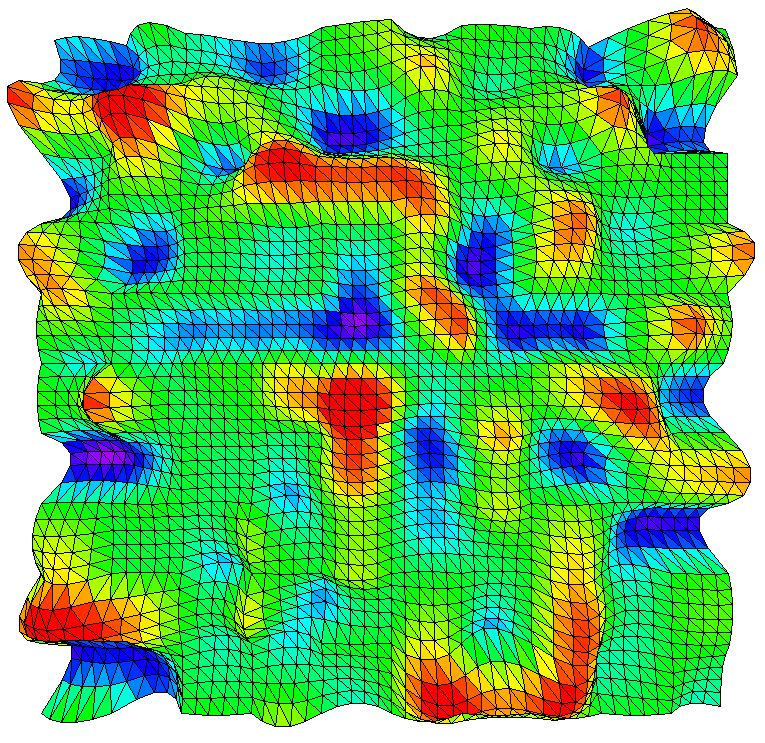
\includegraphics[width=0.95\textwidth]{terrain_01.JPG}
    % }
    % \captionabove{Test}
        % \begin{subfigure}{0.5\textwidth}
        % 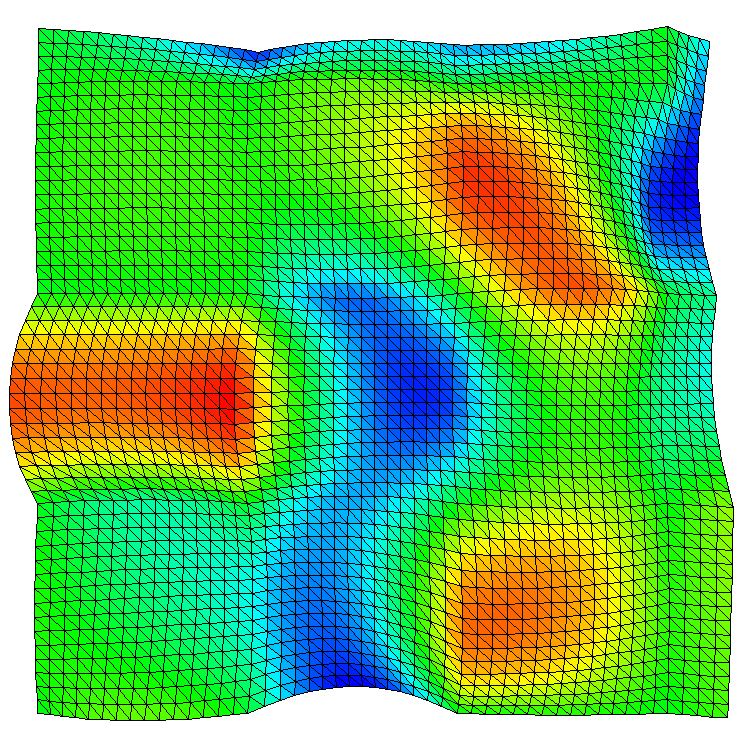
\includegraphics[width=0.95\textwidth, right]{terrain_02.JPG}
        % \caption{Zeitweilig überlagernde Fähigkeiten} \label{img:diayn_ex2}
        % \end{subfigure}
\end{figure}

Wir werden nicht näher auf die Details der Funktion eingehen, da dies nicht Kern dieser Arbeit ist. Für weitere Ausführungen diesbezüglich verweisen wir auf \cite{archer2011procedurally}.

Für die Visualisierung der Landschaft benutzen wir eine abgewandelte Form des Codes von TODO. Zur besseren Differenzierung werden Berge und Täler zusätzlich zur perspektivischen Unterscheidung rot bzw. blau dargestellt.

\smallspace

Wir besitzen nun die Möglichkeit, eine zufällige Landschaft zu generieren und diese visuell darzustellen. Um bei allen Experimenten die gleichen Vorraussetzungen zu gewährleisten, werden wir im folgenden den mittels der eben beschriebenen Methode zufällig generierten Terrain benutzen, der in Abbildung \ref{img:terrainMain} zu sehen ist. Der höchste Punk befindet sich bei dieser Landschaft auf dem Berg ganz oben in der Mitte.

\begin{figure}[h]
    \centering
    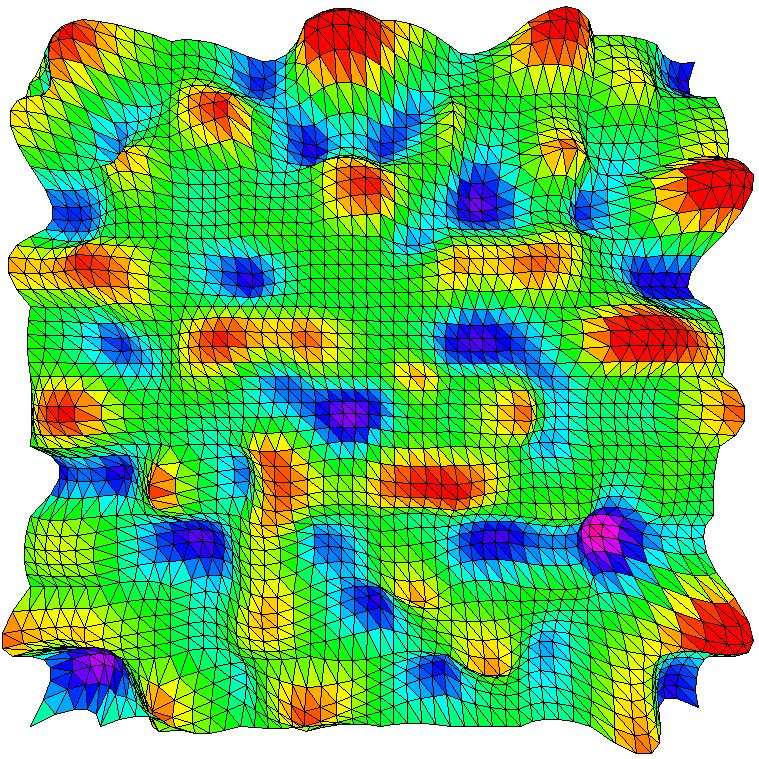
\includegraphics[width=0.5\textwidth, keepaspectratio=true]{terrain_main.JPG}
    \caption{Visualisierung von zweidimensionaler Perlin Noise} \label{img:terrainMain}
\end{figure}

%% Das Environment
\section{Q-Learning}

Um nun zu testen, ob die Landschaft für unsere Zwecke geeignet ist, werden wir einige Experimente durchführen. Wir wollen hierfür zunächst einen simplen Reinforcement Learning Agenten implementieren, welcher \textit{Q-Learning} verwendet.

\subsection{WORKING TITLE: Theory}
% \citeauthor{}

Dieses Kapitel stützt sich zu einem Großteil auf das Buch \textit{Reinforcement Learning: An Introduction, Second Edition} von Sutton u.a. \cite{06_sutton2018reinforcement}. Falls nicht anders angegeben, wurden die Informationen hieraus entnommen.

\paragraph{Policies}
Der Agent folgt zu jedem Zeitpunkt einer Policy $ \pi $. Hierbei gibt $ \pi(a|s) $ die Wahrscheinlichkeit dafür an, dass der Agent zum Zeitschritt $ t $ die Aktion $ a \in A $ im Zustand $ s \in S $ ausführt, also dass $ A_t = a $ wenn $ S_t = s $. Hierbei ist $ S $ die Menge aller Zustände und $ A $ die Menge aller Aktionen. $ \pi(a|s) $ ist also eine Wahrscheinlichkeitsverteilung über $ a \in A(s) $ für jedes $ s \in S $.

\paragraph{State-Value Functions}
Wir benötigen nun eine Möglichkeit einzuschätzen, wie gut ein Zustand $ s $ ist, wenn wir der Policy $ \pi $ folgen. Hierfür nutzen wir die \textit{state-value function} $ v_\pi $. Diese beschreibt die erwartete Belohnung eines Zustands $ s $ unter der Policy $ \pi $ zum Zeitschritt $ t $. Wir definieren $ v_\pi(s) $ als
\begin{align}
    \begin{split}
    v_\pi(s) & \doteq E_\pi \left[G_t | S_t = s \right]\\
    & = E_\pi \left[\sum_{k = 0}^{\infty} \gamma^k R_{t + k + 1} | S_t = s \right],
    \end{split}
\end{align}
wobei $ E_\pi $ der Erwartungswert einer Zufallsvariable ist, gegeben der Agent folgt der Policy $ \pi $.

\paragraph{Action-Value Functions}
Ähnlich hierzu gibt die \textit{action-value function} $ q_\pi $ für die Policy $ \pi $ an, wie profitabel es für den Agenten ist, in einem gegebenen Zustand eine gewisse Aktion auszuführen.

Der Wert einer Aktion $ a $ im Zustand $ s $ unter der Policy $ \pi $ ist also die erwartete Belohnung, wenn man im Zustand $ s $ zum Zeitschritt $ t $ die Aktion $ a $ ausführt. Wir definieren $ q_\pi(s, a) $ als
\begin{align}
    \begin{split}
    q_\pi(s,a) & \doteq E_\pi \left[G_t | S_t = s, A_t = a \right]\\
    & = E_\pi \left[\sum_{k = 0}^{\infty} \gamma^k R_{t + k + 1} | S_t = s, A_t = a \right].
    \end{split}
\end{align}
Die action-value function wird auch als Q-function bezeichnet, welche als Ergebnis für ein state-action Paar die Q-value liefert. Für die folgenden Implementierungen ist diese von großer Wichtigkeit.

\paragraph{Optimale Policies und Optimale Value Functions}
Das Ziel des Agenten ist, die optimale Policy $ \pi $ für ein Markov Decision Problem zu finden. Ist dieses Ziel erreicht so lässt sich sagen, dass die Reinforcement Learning Aufgabe erfüllt ist. Optimal ist hierbei die Policy, welche nach Aufsummieren der Belohnungen über alle Schritte einer Episode die beste gesamte Belohnung liefert. Eine Policy $ \pi $ ist also besser als Policy $ \pi' $, wenn die erwartete Belohnung von $ \pi $ für \textbf{alle} Zustände $ s \in S $ größer ist als die von $ \pi' $. \cite{06_sutton2018reinforcement} verwendet die Formulierung
\begin{align}
    \pi \geq \pi' \text{ if and only if } v_\pi(s) \geq v_{\pi'}(s) \text{ for all } s \in S.
\end{align}

Es gibt immer eine Policy, die besser als oder gleichwertig mit allen anderen Policies ist. Diese wird beziehungsweise werden als $ \pi_* $ bezeichnet. Die besten Policies besitzen die gleich state-value function, welche die \textit{optimale state-value function} $ v_* $ genannt wird und definiert wird als
\begin{align}
    v_*(s) \doteq \max_\pi v_\pi(s)
\end{align}
für alle $ s \in S $.

Optimale Policies teilen sich ebenfalls die gleiche \textit{optimale action-value function} $ q_* $, welche definiert ist als
\begin{align}
    q_*(s, a) \doteq \max_\pi q_\pi(s, a)
\end{align}
für alle $ s \in S $ und $ a \in A $. $ q_* $ liefert also für jedes state-action Paar den größtmöglichen erwarteten Ertrag, den irgendeine Policy erreichen kann.

\paragraph{Bellman Optimality Equasion}
Die optimale action-value function $ q_* $ muss die folgende Gleichung erfüllen:
\begin{align}
    q_*(s, a) = E \left[R_{t + 1} + \gamma \max_{a'} q_*(s', a') \right]
\end{align}
Diese Gleichung wird \textit{Bellman optimality equation} für $ q_* $ genannt und besagt, dass der beste erwartete Ertrag für jedes state-action Paar $ (s, a) $ zum Zeitpunkt $ t $ der Summe aus der direkten Belohnung $ R_{t + 1} $ der Aktion $ a $ und dem \textbf{maximalen} erwarteten Ertrag, der von einem der nächsten state-action Paare $ (s', a') $ erreicht werden kann, mit discount $ \gamma $ entsprechen muss.

Wir werden die Bellman equasion verwenden, um $ q_* $ zu finden. $ q_* $ wiederum liefert uns die optimale Policy.

\subsection{Implementierung in Python}

% \begin{figure}[h]
%     \centering
%     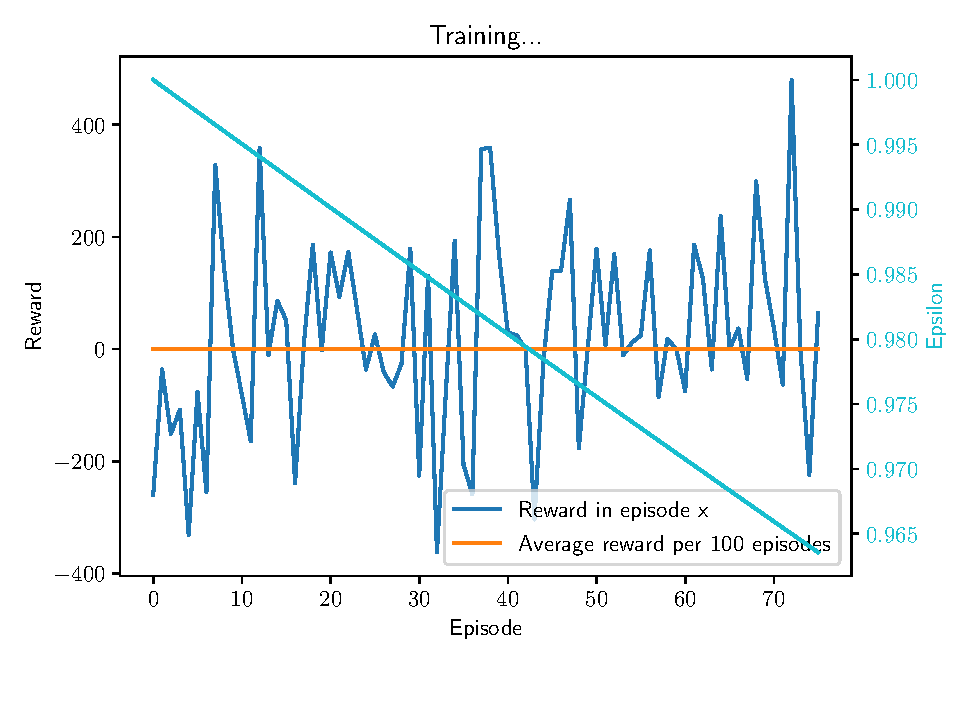
\includegraphics[width=\textwidth]{plot_test.pdf}
%     \caption{Visualisierung von zweidimensionaler Perlin Noise} \label{img:terrainMain}
% \end{figure}

% \begin{align}
%     \mathcal{F}(\theta) & = H(A|S,Z) - H(Z|S) + H(Z) \nonumber\\
%     & = H(A|S,Z) + E_{z \sim p(z), s \sim \pi(z)}(log\ p(z | s)) - E_{z \sim p(z)}(log\ p(z)) \label{eq:objective_2}\\
%     & \ge H(A|S,Z) + E_{z \sim p(z), s \sim \pi(z)}(log\ q_\phi(z | s) - log\ p(z)) \stackrel{\triangle}{=} \mathcal{G}(\theta, \phi) \nonumber
% \end{align}


% Grid, auf dem sich der Agent bewegen
% Perlin Noise
% 
% Color-coded: Rot ist hoch, blau ist tief
% 

%% Ziel des Agenten

%% Agent mit Q-Table

%% Agent mit Neuronalem Netz

%% Ergebnisse

% \begin{minted}{python}
%     import numpy as np
      
%     def incmatrix(genl1,genl2):
%         m = len(genl1)
%         n = len(genl2)
%         M = None #to become the incidence matrix
%         VT = np.zeros((n*m,1), int)  #dummy variable
      
%         #compute the bitwise xor matrix
%         M1 = bitxormatrix(genl1)
%         M2 = np.triu(bitxormatrix(genl2),1) 
      
%         for i in range(m-1):
%             for j in range(i+1, m):
%                 [r,c] = np.where(M2 == M1[i,j])
%                 for k in range(len(r)):
%                     VT[(i)*n + r[k]] = 1;
%                     VT[(i)*n + c[k]] = 1;
%                     VT[(j)*n + r[k]] = 1;
%                     VT[(j)*n + c[k]] = 1;
      
%                     if M is None:
%                         M = np.copy(VT)
%                     else:
%                         M = np.concatenate((M, VT), 1)
      
%                     VT = np.zeros((n*m,1), int)
      
%         return M
%     \end{minted}